\chapter{Estado del Arte}

\subsection{Aplicaciones de rastreo para familia y amigos}

Actualmente las redes sociales forman parte de nuestra vida cotidiana, desde la posibilidad de enviar un mensaje privado, hasta la posibilidad de capturar en tiempo real nuestras historias y compartirlas con nuestra comunidad de amigos, entre muchas otras características. De esta manera las redes sociales ha logrado penetrar en lo más profundo del tejido social.

Así mismo, buscamos obtener la mayor experiencia de uso, apoyándonos de todas las posibles herramientas multimedia que existen. Tales como: texto, imágenes, voz, video, storytelling etc. y por supuesto recientemente el poder compartir nuestra ubicación en vivo con familiares y amigos.

De esta manera resolvemos la problemática que tenían los usuarios para reunirse en el mundo real. Ya sea que se esté compartiendo un viaje, que le informemos a nuestros seres queridos que hemos llegado a salvo, o reunirnos con nuestros amigos. Estas son experiencias muy comunes para todos nos otros. \cite{zafirKhan}

Es por  esto que las principales aplicaciones móviles han optado por  integrar esta caracteristica. 

Cabe mencionar que estamos aprovechamos el sistema de localización más exacto y preciso que existe y lo llevamos a nuestras interacciones humanas, para volverlas aún más emotivas y gratificantes.

\subsubsection{WhatsApp Live Location}

asd

\subsubsection{Find My Friends - Apple}

Es una aplicación gratuita propiedad de Apple Inc. Está enfocada en la localización de familiares o amigos.

\begin{figure}[bp!]
	\centering
	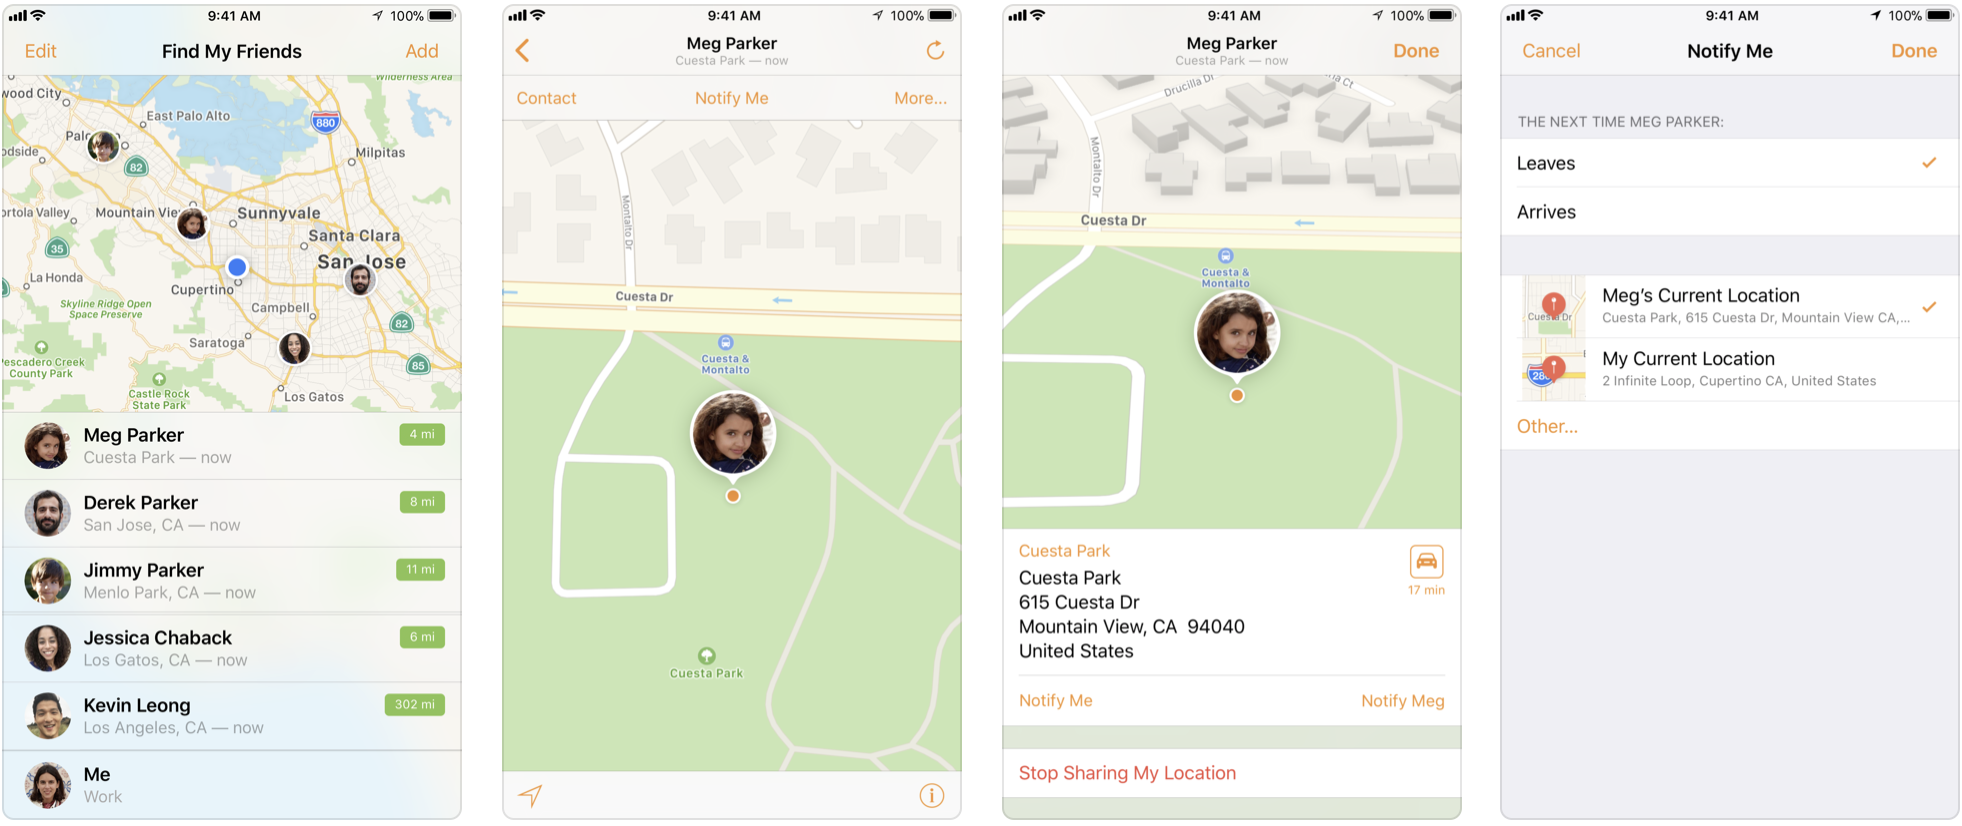
\includegraphics[width=5in]{imgs/apple_findmyfriends}
	  \caption{Find My Friends}
\end{figure}

``Find My Friends" version 7.0 requiere iOS 11 o posterior así como una cuenta de iCloud. Es compatible tanto para iPhone, iPad o iPod touch.

El primer paso es agregar contactos a nuestra aplicación enviando una solicitud a su dirección de correo asociada al iCloud del dispositivo, también es posible agregarlos a través de su número de teléfono igualmente asociado a su cuenta de iCloud o usando AirDrop (localizador de terminales Apple en un perímetro cercano, a través de bluethoot y la red wifi).

Posterior a eso tendremos que esperar a que acepte nuestra solicitud.

Una vez aceptada la solicitud ya forma parte de nuestros contactos. Ahora podremos compartir nuestra ubicación actual, así mismo nuestros contactos pueden empezar a seguir nuestra ubicación inmediatamente, también ellos pueden compartir sus ubicaciones. Si en algún momento se desea dejar de compartir la ubicación, basta con mover un interruptor para dejar de compartirla.

Una característica interesante y que agrega gran valor, son las notificaciones de geocercas (perímetros des algún punto/ubicación en especifico). Por ejemplo tiene la capacidad de notificar cuando un amigo llega al aeropuerto, cuando un niño sale de la escuela o un miembro de la familia llega a casa de manera segura. \cite{findmyfriends}

A continuación se muestran algunas ventajas y desventajas de la aplicación:

\paragraph{Ventajas}

\begin{itemize}
    \item ``Find My Friends" no almacena de manera permanente la información de nuestra ubicación.
    \item En la mayoría de los casos viene pre instalada.
    \item No necesita un registro ya que toma las credenciales de nuestra cuenta de iCloud asociada a nuestros dispositivo.
    \item Además de nuestra terminal física, se puede monitorear a nuestros contactos desde un navegador web, desde iCloud.com
    \item Se puede usar el Apple Watch (con WatchOS 3 o superior) para compartir la ubicación.
    \item Notificación de geocercas, entradas y salidas de nuestros amigos en un punto dado.
\end{itemize}

\paragraph{Desventajas}

\begin{itemize}
\item Tus amigos o familia deben tener un dispositivo Apple (iPhone, iPad, iPod).
\item En el día a día es común olvidar desactivar compartir ``ubicación", esto permite que tus contactos puedan ver tu ubicación actual permanentemente.
\item Si tus amigos dejan de compartir su ubicación, necesitas solicitarles compartan su ubicación y esperar a que lo hagan. Aun que se puede hacer desde la aplicación por lo general terminas solicitándolo desde otros medios.
\item Sólo un dispositivo envía la ubicación, es decir si tengo 2 iPhones y 1 Apple Watch sólo 1 de ellos puede compartir la ubicación con mis amigos. Sin opción de configurarlo.
\end{itemize}

En resumen al integrar todo el ecosistema de Apple se logra una gran calidad el funcionamiento de la aplicación, sin embargo también se vuelve muy dependiente de éste volviéndolo también su principal desventaja.